\documentclass{beamer}

\usetheme{Boadilla}
\usecolortheme{dove}

\usepackage{graphicx}
\usepackage{hyperref}
\usepackage{booktabs}
\usepackage{textcomp}
\usepackage{gensymb}
\usepackage{float}
\graphicspath{{../figures/}}

\title{
  Studying the Effect of Natural Disasters on Economic Activity:\\
  \large{A first Approach using Night-Time Luminosity Data}
}
\author{Cameron, M. \and Rosales, V. \and Westermann, J.P.}

\date{July 30, 2017}

\begin{document}

\begin{frame}
  \maketitle
\end{frame}

\begin{frame}{Modelling Earthquake Impact}{Linearly Decaying with Distance}
  \begin{figure}
    \centering
    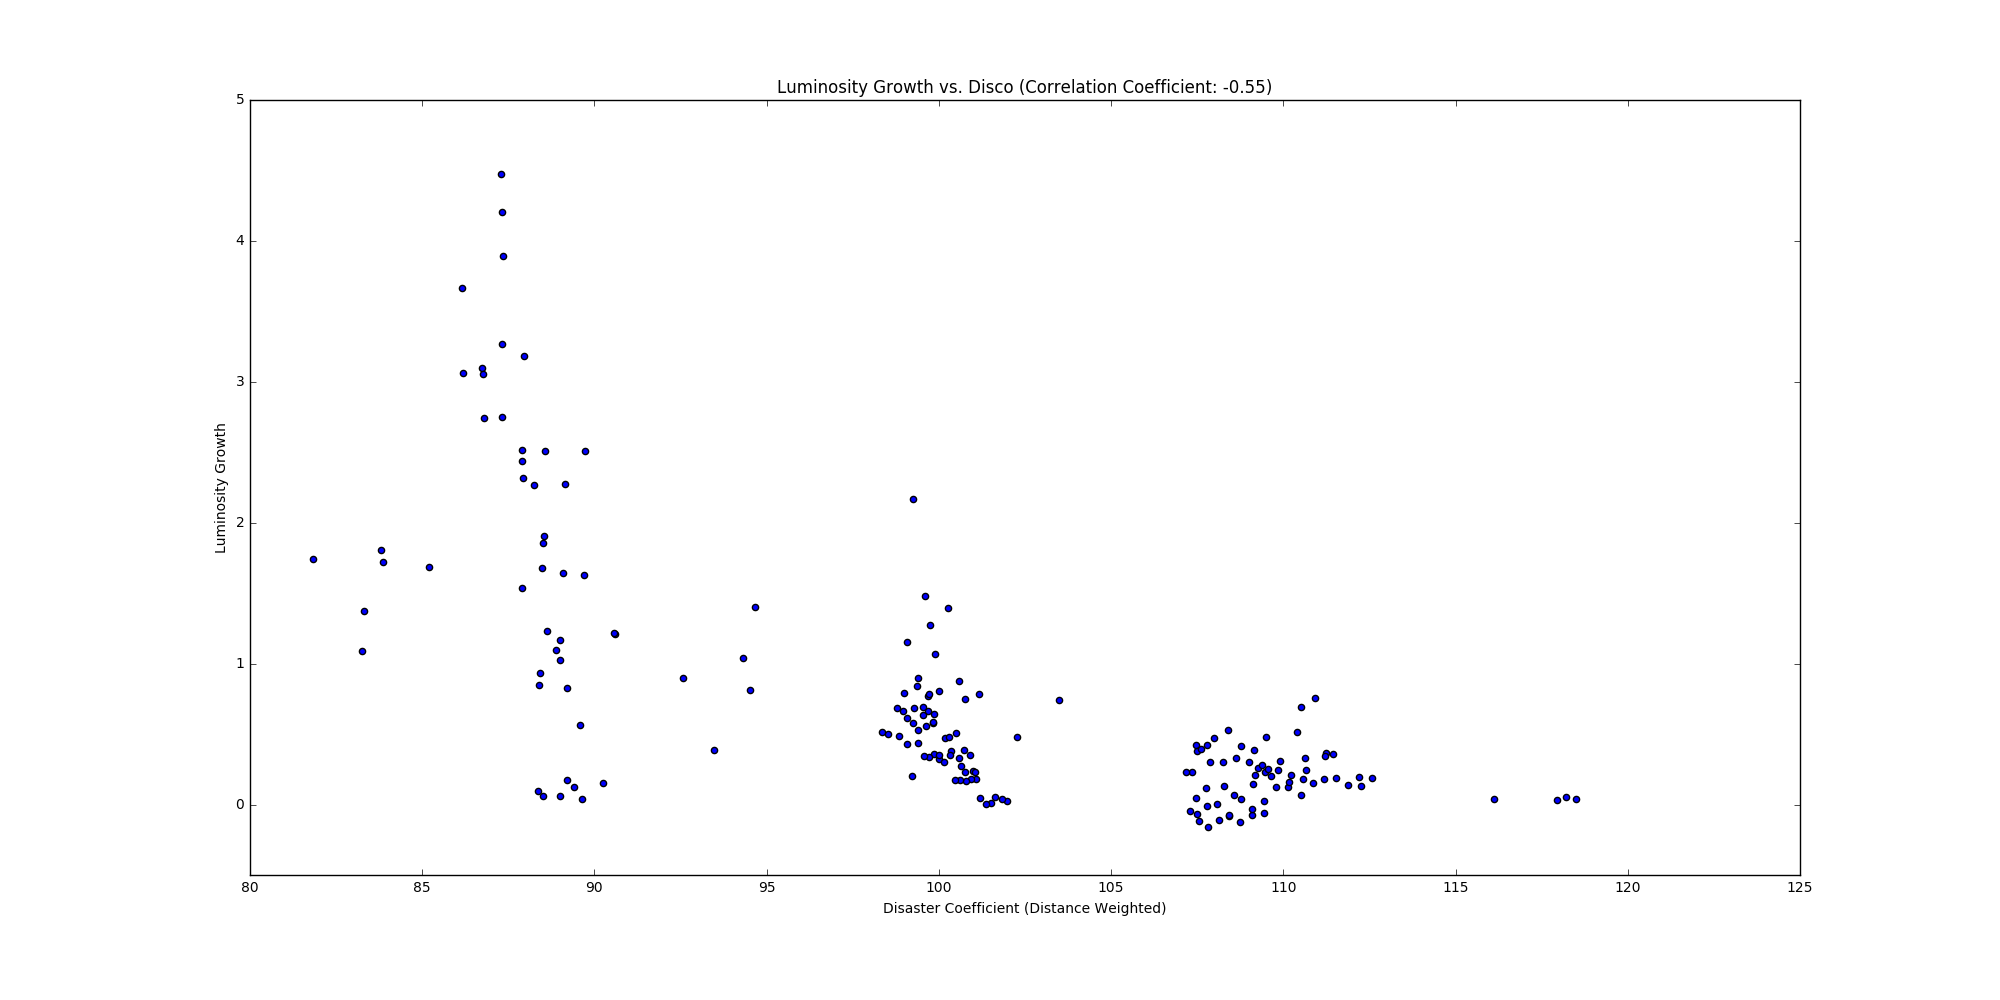
\includegraphics[height=1\paperheight]{linear-lum-vs-disco}\label{fig:linear-model-disco-vs-lum-growth} %TODO: Adjust plot pngs to have sensible size for document
    \caption{Luminosity Growth 1992-2013 plotted against a linearly decaying disaster coefficient for 150x150 image sections.}
  \end{figure}
\end{frame}

\begin{frame}{Modelling}
    \begin{center}
      \begin{tabular}{lr}\\
        \toprule
        {} & Average Coefficient \\
        \midrule
        el1 & -0.60 \\
        el2 & -0.37 \\
        el3 & -0.14 \\
        \bottomrule\\
      \end{tabular}\\
    \end{center}
  \end{block}
\end{frame}

% \begin{frame}
%   \begin{block}{Panel Model}
%     \begin{figure}
%       \centering
%       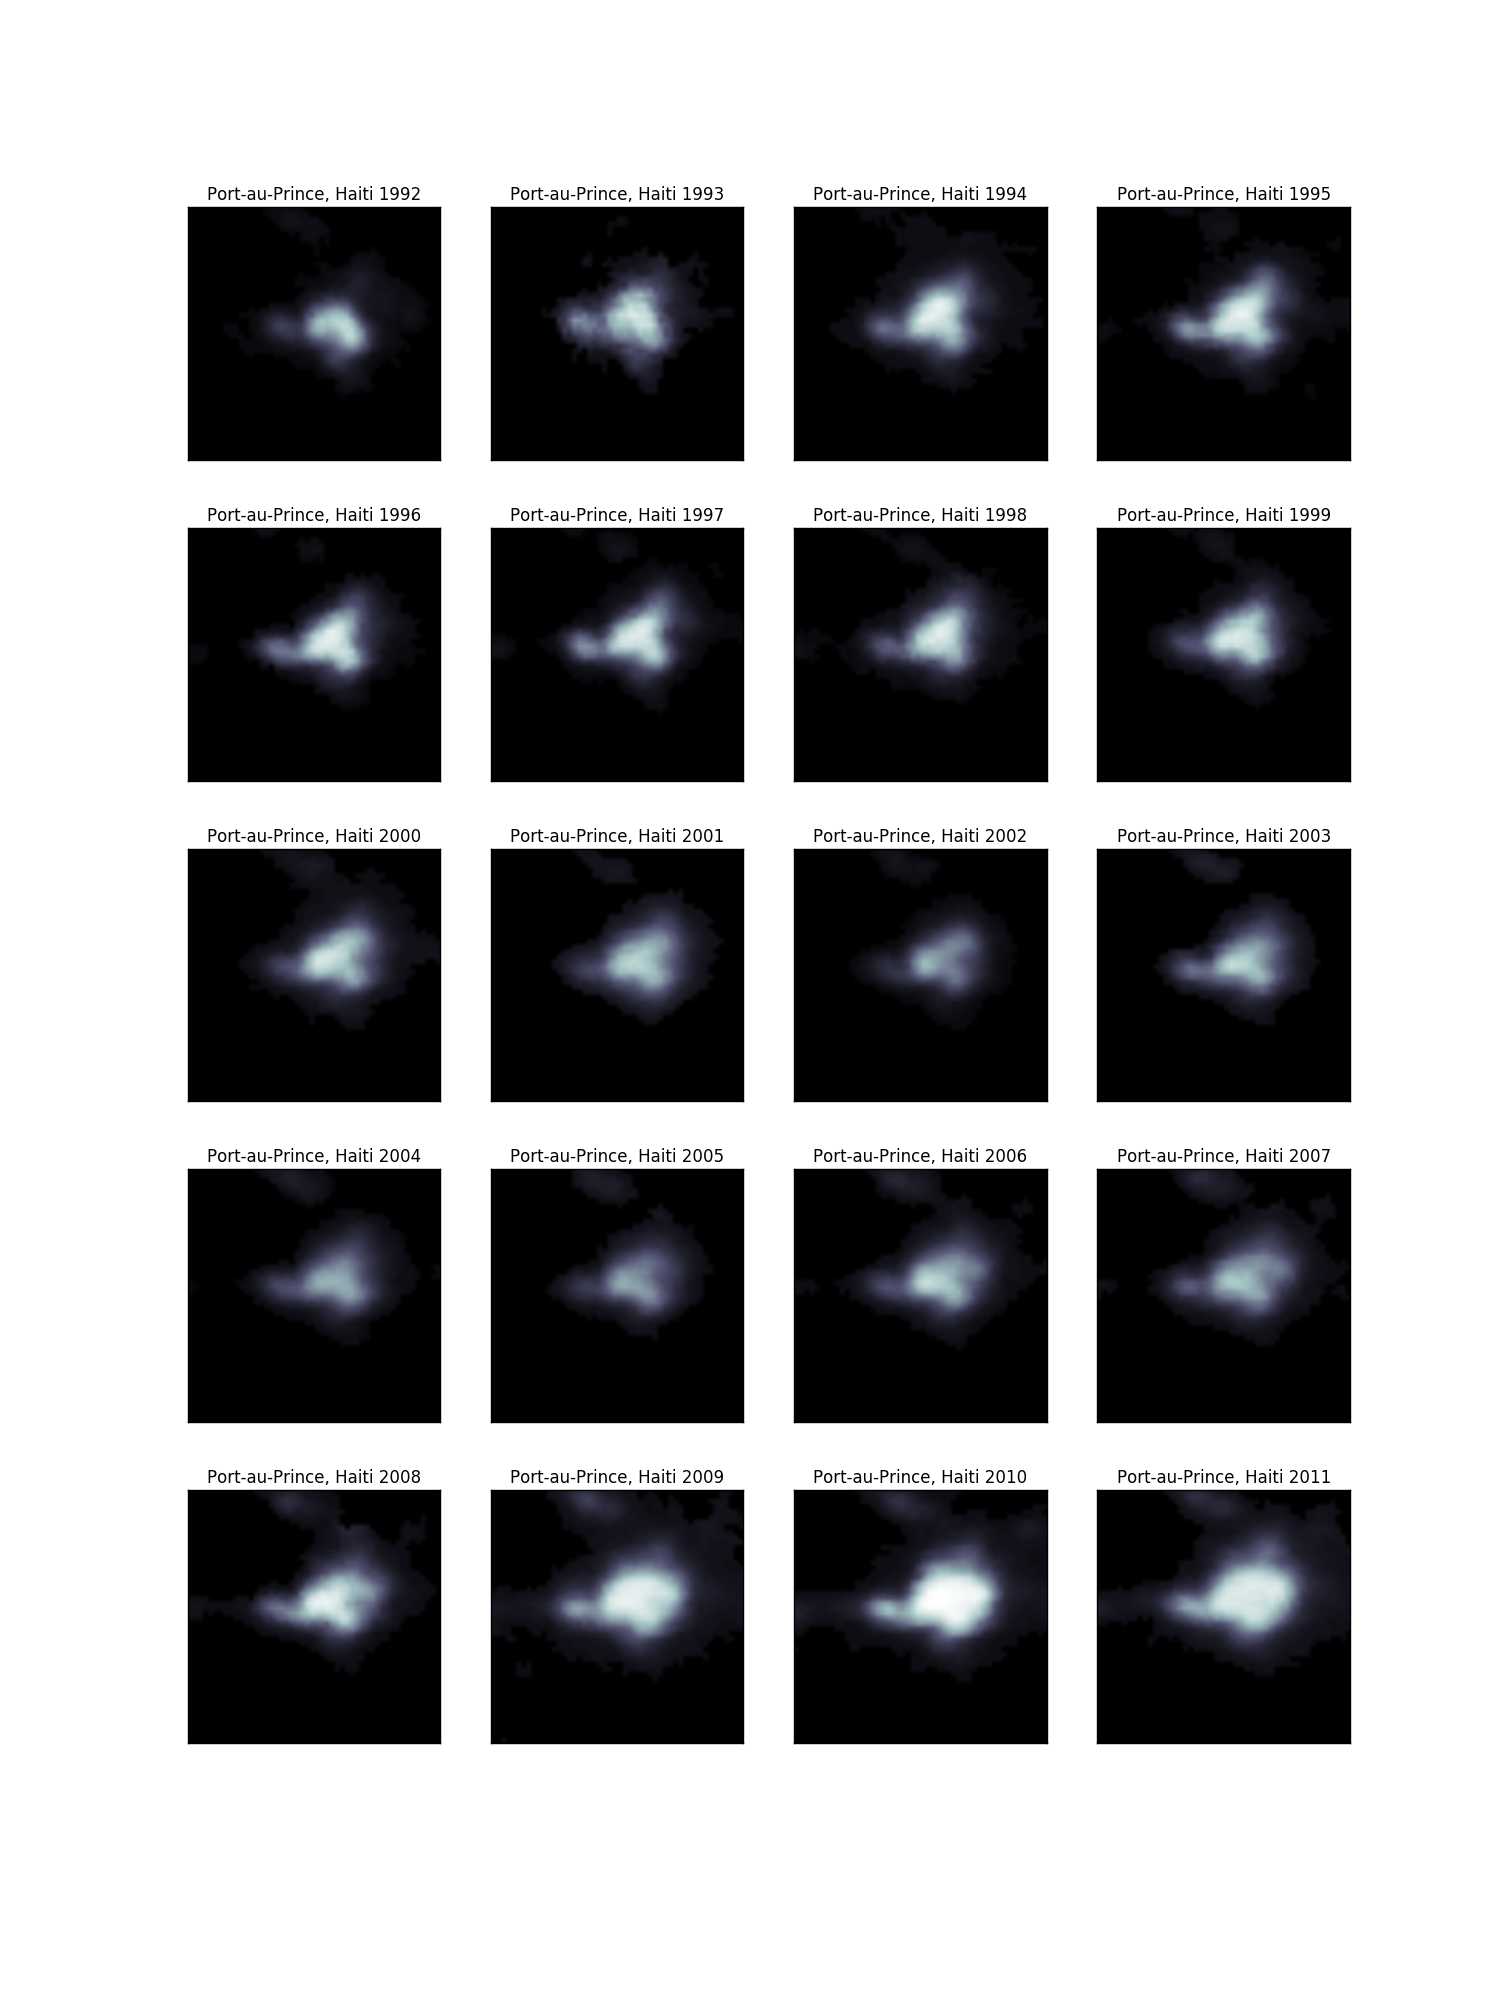
\includegraphics[width=\linewidth]{haiti_luminosity_series}\label{fig:haiti_luminosity_series}
%       \caption{50x50 pixel atellite image cutout of Port-au-Prince, Haiti}
%     \end{figure}
%     \begin{figure}[H]
%       \centering
%       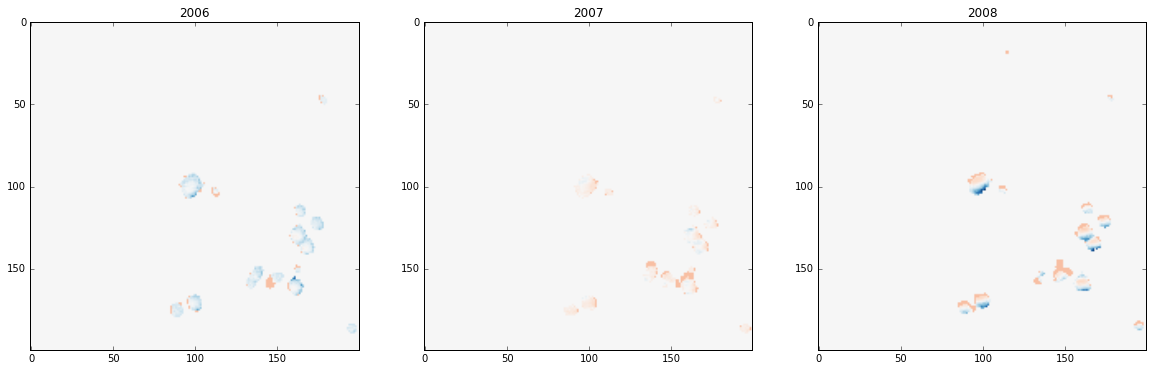
\includegraphics[width=1\linewidth]{tocopilla_series}\label{fig:tocopilla_series}
%       \caption{Absolute change in luminosity in Tocopilla}
%       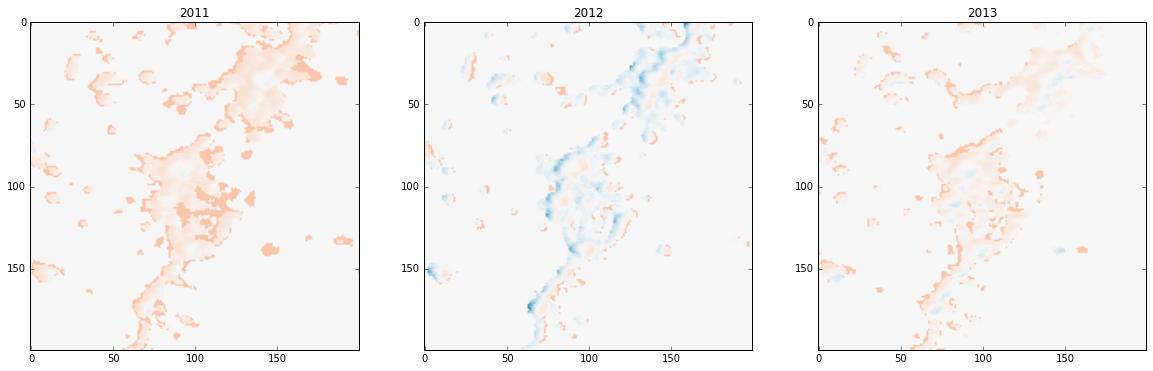
\includegraphics[width=1\linewidth]{maule_series}\label{fig:maule_series}
%       \caption{Absolute change in luminosity in Maule}
%     \end{figure}
%     \begin{figure}[H]
%     \centering
%       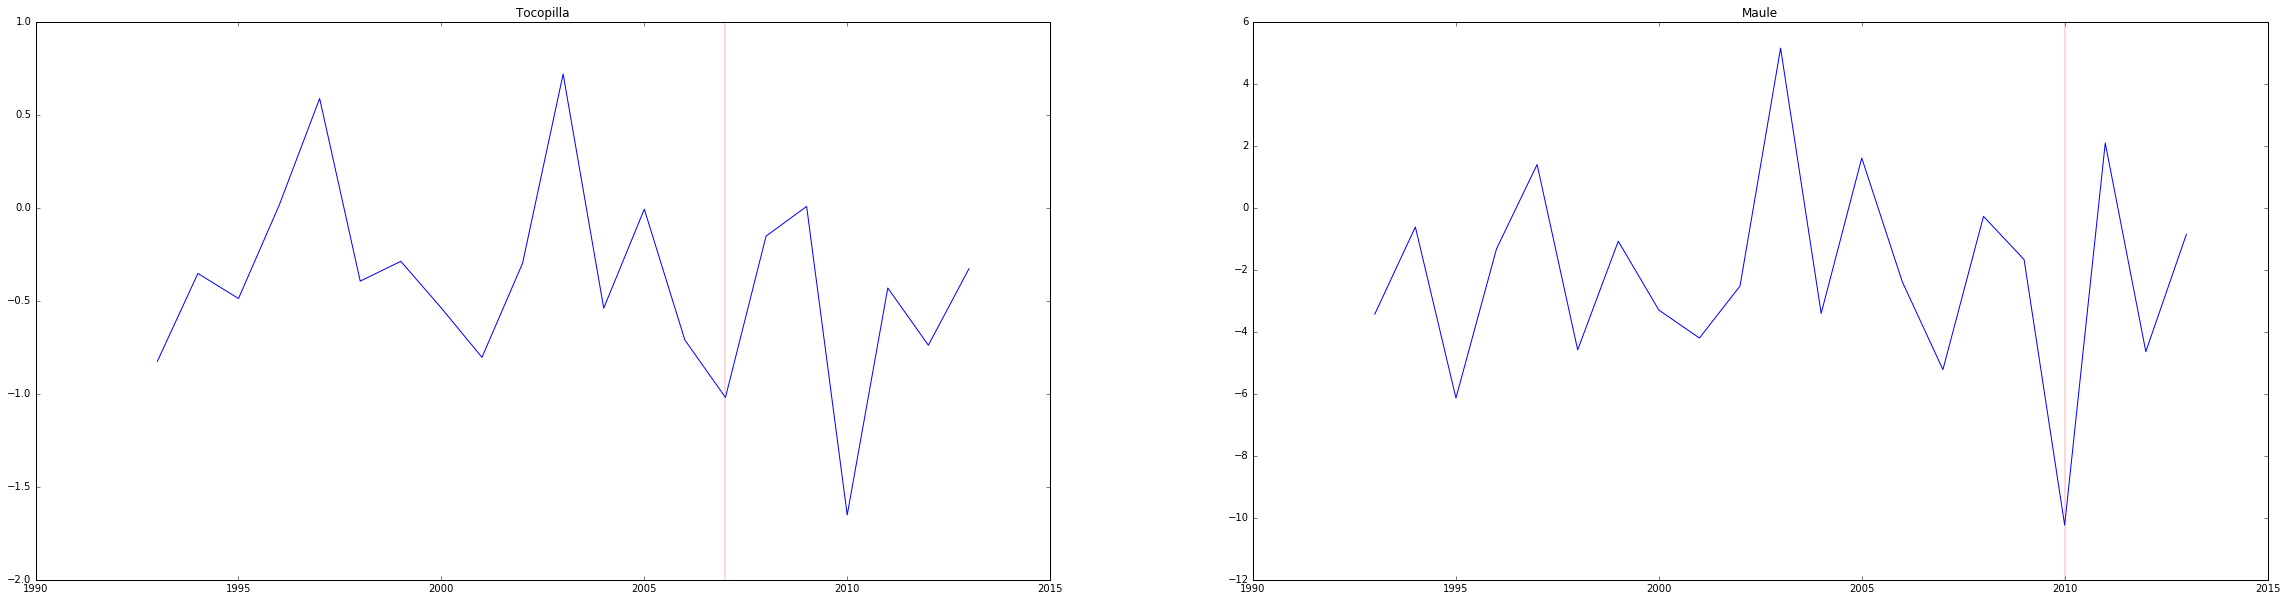
\includegraphics[width=1\linewidth]{maule_tocopilla}\label{fig:maule_tocopilla}
%     \end{figure}
%     \begin{figure}[H]
%       \centering
%       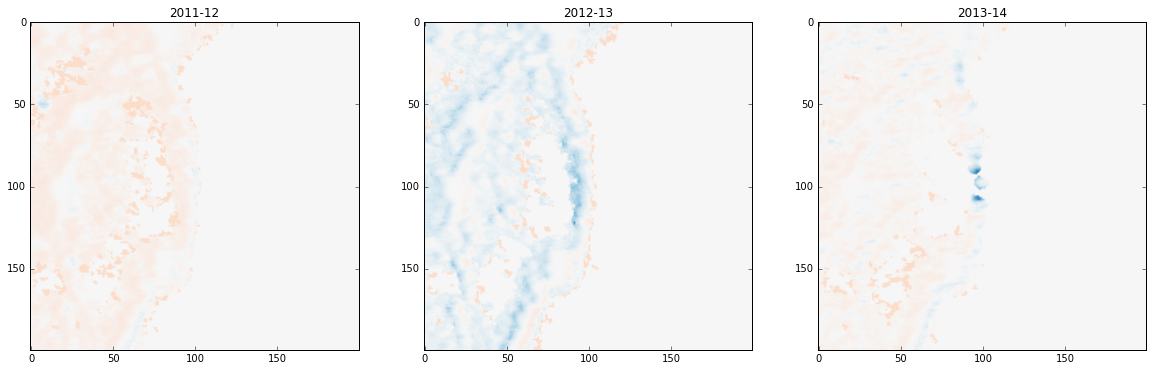
\includegraphics[width=1\linewidth]{fukushima}\label{fig:fukushima}
%     \end{figure}
% \end{frame}

\begin{thebibliography}{9}
	\bibitem{lightasproxy} 
	Xi Chen and William D. Nordhausn. 
	\textit{Using luminosity data as a proxy for economic statistics}. 
	Proceedings of the National Academy of Sciences, 2010.

	\bibitem{lightcamera} 
	Maxim Pinkovskiy and Xavier Sala-i-Martin. 
	\textit{Lights, Camera,...Income! Estimating Poverty Using National Accounts, Survey Means, and Lights}. 
	NBER WP 19831, 2014.

	\bibitem{growthlights} 
	VJ Henderson, A Storeygard and Weil DN. 
	\textit{Measuring Economic Growth from Outer Space}. 
	American Economic Review, 2011.

	\bibitem{africalights} 
	Stelios Michalopoulos and Elias Papaioannou. 
	\textit{Pre-colonial Ethnic Institutions and Contemporary African Development}. 
	Econometrica, 2013 Jan; 81(1): 113–152.

	\bibitem{houserates} 
	Chilean Ministry of Planning . 
	\textit{Encuesta Post Terremoto: Principales resultados}. 
	Ministerio de Planificación, 2011.
\end{thebibliography}

\end{document}
